\subsection*{题目背景}

小 H 同学发现,他维护的存储系统经常出现有人用机器学习的训练数据把空间占满的问题,十分苦恼。
查找了一阵资料后,他想要在文件系统中开启配额限制,以便能够精确地限制大家在每个目录中最多能使用的空间。

\subsubsection*{文件系统概述}

文件系统,是一种树形的文件组织和管理方式。在文件系统中,{\heiti{文件}}是指用名字标识的文件系统能够管理
的基本对象,分为{\heiti{普通文件}}和{\heiti{目录文件}}两种,目录文件可以被简称为 {\heiti{目录}}。目录中有一种特殊的目录被叫做{\heiti{根目录}} 。
除了根目录外,其余的文件都有名字,称为{\heiti{文件名}}。合法的文件名是一个由若干数字(\verb|[0-9]|)、
大小写字母(\verb|[A-Za-z]|)组成的非空字符串。普通文件中含有一定量的数据,占用存储空间;目录不占用存储空间。
文件和目录之间存在{\heiti{含于}}关系。上述概念满足下列性质:

\begin{enumerate}

    \item 有且仅有一个{\heiti{根目录}};

    \item 对于除根目录以外的文件,都含于且恰好含于一个目录;

    \item 含于同一目录的文件,它们的文件名互不相同;

    \item 对于任意不是根目录的文件 $f$,若 $f$ 不含于根目录,那么存在有限个目录 $d_1, d_2, \dots, d_n$,
          使得 $f$ 含于 $d_1$,$d_1$ 含于 $d_2$,$\dots$,$d_n$ 含于根目录。

\end{enumerate}

结合性质 4 和性质 2 可知,性质 4 中描述的有限多个目录,即诸 $d_i$,是唯一的。再结合性质 3,
我们即可通过从根目录开始的一系列目录的序列,来唯一地指代一个文件。我们记任意不是根目录且不含于
根目录的文件 $f$ 的文件名是 $N_f$,那么 $f$ 的{\heiti{路径}} 是:$‘/’ + N_{d_n} + ‘/’ +
    \dots + N_{d_1} + ‘/’ + N_f$,其中符号 $+$ 表示字符串的连接;对于含于根目录的文件 $f$,
它的路径是:$‘/’ + N_f$;根目录的路径是:$‘/’$。不符合上述规定的路径都是非法的。例如:\verb|/A/B|
是合法路径,但 \verb|/A//B|、\verb|/A/|、\verb|A/|、\verb|A/B| 都不是合法路径。

若文件 $f$ 含于目录 $d$,我们也称 $f$ 是 $d$ 的{\heiti{孩子文件}}。$d$ 是 $f$ 的{\heiti{双亲目录}}。
我们称文件 $f$ 是目录 $d$ 的{\heiti{后代文件}},如果满足:(1) $f$ 是 $d$ 的孩子文件,或(2)
$f$ 含于 $d$ 的后代文件。

\begin{figure}[H]
    \centering
    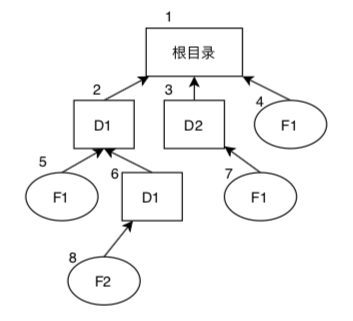
\includegraphics[width=0.5\textwidth]{image/21/3-p-1.png}
\end{figure}

如图所示,该图中绘制的文件系统共有 8 个文件。其中,方形表示目录文件,圆形表示普通文件,它们之间
的箭头表示含于关系。在表示文件的形状上的文字是其文件名;各个形状的左上方标记了序号,以便叙述。
在该文件系统中,文件 5 含于文件 2,文件 5 是文件 2 的孩子文件,文件 5 也是文件 2 的后代文件。
文件 8 是文件 2 的后代文件,但不是文件 2 的孩子文件。文件 8 的路径是 \verb|/D1/D1/F2|。

\subsubsection*{配额概述}
配额是指对文件系统中所含普通文件的总大小的限制。
对于每个目录 $d$,都可以设定两个配额值:{\heiti{目录配额}}和
{\heiti{后代配额}}。我们称目录配额 $LD_{d}$ 是{\heiti{满足的}},当且仅当 $d$ 的孩子文件中,
全部普通文件占用的存储空间之和不大于该配额值。我们称后代配额 $LR_{d}$
是{\heiti{满足的}},当且仅当 $d$ 的后代文件中,全部普通文件占用的存储空间之和不大于该配额值。
我们称文件系统的配额是满足的,当且仅当该文件系统中所有的配额都是满足的。

很显然,若文件系统中仅存在目录,不存在普通文件,那么该文件系统的配额一定是满足的。随着配额和文件
的创建,某个操作会使文件系统的配额由满足变为不满足,这样的操作会被拒绝。例如:试图设定少于目前已有
文件占用空间的配额值,或者试图创建超过配额值的文件。

\subsection*{题目描述}

在本题中,假定初始状态下,文件系统仅包含根目录。你将会收到若干对文件系统的操作指令。对于每条指令,
你需要判断该指令能否执行成功,对于能执行成功的指令,在成功执行该指令后,文件系统将会被相应地修改。
对于不能执行成功的指令,文件系统将{\heiti{不会发生任何变化}}。你需要处理的指令如下:

\subsubsection*{创建普通文件}

创建普通文件指令的格式如下:

\begin{lstlisting}
C <file path> <file size>
\end{lstlisting}

创建普通文件的指令有两个参数,是空格分隔的字符串和一个正整数,分别表示需要创建的普通文件的路径和
文件的大小。

对于该指令,若路径所指的文件已经存在,且也是普通文件的,
则替换这个文件;若路径所指文件已经存在,但是目录文件的,则该指令不能执行成功。

当路径中的任何目录不存在时,应当尝试创建这些目录;若要创建的目录文件与已有的同一双亲目录下的孩子
文件中的普通文件名称重复,则该指令不能执行成功。

另外,还需要确定在该指令的执行是否会使该文件系统的
配额变为不满足,如果会发生这样的情况,则认为该指令不能执行成功,反之则认为该指令能执行成功。

\subsubsection*{移除文件}

移除文件指令的格式如下:

\begin{lstlisting}
R <file path>
\end{lstlisting}

移除文件的指令有一个参数,是字符串,表示要移除的文件的路径。

若该路径所指的文件不存在,则不进行任何操作。

若该路径所指的文件是目录,则移除该目录及其所有后代文件。

在上述过程中被移除的目录(如果有)上设置的配额值也被移除。

该指令始终认为能执行成功。

\subsubsection*{设置配额值}

\begin{lstlisting}
Q <file path> <LD> <LR>
\end{lstlisting}

设置配额值的指令有三个参数,是空格分隔的字符串和两个非负整数,分别表示需要设置配额值的目录
的路径、目录配额和后代配额。

该指令表示对所指的目录文件,
分别设置目录配额和后代配额。若路径所指的文件不存在,或者不是目录文件,则
该指令执行不成功。

若在该目录上已经设置了配额,则将原配额值替换为指定的配额值。

特别地,若配额值为 0,
则表示不对该项配额进行限制。若在应用新的配额值后,该文件系统配额变为不满足,那么该指令执行不成功。


\subsection*{输入格式}

从标准输入读入数据。

输入的第一行包含一个正整数 $n$,表示需要处理的指令条数。

输入接下来会有 $n$ 行,每一行一个指令。指令的格式符合前述要求。输入数据保证:对于所有指令,
输入的路径是合法路径;对于创建普通文件和移除文件指令,输入的路径不指向根目录。


\subsection*{输出格式}

输出到标准输出。

输出共有 $n$ 行,表示相应的操作指令是否执行成功。若成功执行,则输出字母 \verb|Y|;否则输出 \verb|N|。

\examplebox*{\lstinputlisting[frame=none]{data/21/3-1.in}}{\lstinputlisting[frame=none]{data/21/3-1.out}}

输入总共有 10 条指令。其中前两条指令可以正常创建两个普通文件。第三条指令试图创建 /A/B/1/3,
但是 /A/B/1 已经存在,且不是目录,而是普通文件,不能再进一步创建孩子文件,因此执行不成功。
第四条指令试图创建 /A,但是 /A 已经存在,且是目录,因此执行不成功。第五条指令试图删除 /A/B/1/3,
由于该文件不存在,因此不对文件系统进行修改,但是仍然认为执行成功。第六条指令试图在根目录
增加后代配额限制,但此时,文件系统中的文件总大小是 2048,因此该限制无法生效,执行不成功。
第七条指令试图创建文件 /A/B/1,由于 /A/B/1 已经存在,且是普通文件,因此该指令实际效果是
将原有的该文件替换。此时文件总大小是 1124,因此第八条指令就可以执行成功了。
第九条指令递归删除了 /A/B 目录和它的所有后代文件。此时文件系统中已经没有普通文件,因此第十条命令
可以执行成功。

\examplebox*{\lstinputlisting[frame=none]{data/21/3-2.in}}{\lstinputlisting[frame=none]{data/21/3-2.out}}

输入共有 9 条指令。第一条指令试图为 /A/B 创建配额规则,然而该目录并不存在,因此执行不成功。
接下来的两条指令创建了两个普通文件。再接下来的两条指令分别在目录 /A/B 和 /A/C 创建了
两个配额规则。其中前者是目录配额,后者是后代配额。接下来的两条指令,创建了
两个文件。其中,/A/B/3 超出了在 /A/B 的目录配额,因此执行不成功;但 /A/B/D/3
不受目录配额限制,因此执行成功。最后两条指令,创建了两个文件。虽然在 /A/C
没有目录配额限制,但是无论是 /A/C 下的孩子文件还是后代文件,都受到后代配额的限制,因此两条指令
执行都不成功。

\subsection*{子任务}

本题目各个测试点的数据规模如下:

\begin{table}[H]
    \centering
    \begin{tabular}{c|c|c|c|c|c}
        % \toprule
        \thickhline
        测试点   & 操作数                      & 单个文件大小                & 路径长度                   & 目录层次                  & 没有操作 $Q$ \\ \hline
        % \midrule
        $1,2$    & \multirow{2}{*}{$\le 100$}  & \multirow{4}{*}{$\le 10^9$} & \multirow{4}{*}{$\le 100$} & \multirow{4}{*}{$\le 20$} & 是           \\ \cline{1-1} \cline{6-6}
        $3,4$    &                             &                             &                            &                           & 否           \\ \cline{1-2} \cline{6-6}
        $5,6,7$  & \multirow{2}{*}{$\le 10^5$} &                             &                            &                           & 是           \\ \cline{1-1} \cline{6-6}
        $8,9,10$ &                             &                             &                            &                           & 否           \\ \thickhline
        % \bottomrule
    \end{tabular}
\end{table}

表格中,目录层次是指各指令中出现的路径中,\verb|/| 字符的数目。

所有输入的数字均不超过$10^{18}$。


